\chapter{Theoretical Framework}\label{theoretical-framework}

\begin{itemize}
\itemsep1pt\parskip0pt\parsep0pt
\item
  Static Analysis tools as cmd line tools
\item
  How can they help integrated into the text editor?
\end{itemize}

This chapter will introduce the research done prior to the design. It
will explain the motivation behind working on software development
environments, give a short history of \glspl{ide} and list typical
\gls{ui} design patterns in \glspl{ide}. It will close by presenting a
survey and a series of interviews done in order to understand the
problem space.

\section{History and role of IDEs}\label{history-and-role-of-ides}

Software development environments have been predecessed by general text
editors, starting with several projects at the Xerox \gls{parc}. Douglas
Engelbart created the text editor for the NLS system (oNLine System)
which allowed \gls{wysiwyg} style editing \cite[pp.]{moggridge}. In the
\emph{Gypsy} text editor, Larry Tesler first integrated modeless moving
of text, which is known as \emph{Copy\&Paste} \cite[pp.]{moggridge}.
Text editors with those functionalities are now the core of any software
development environment.

Later, while working with Alan Kay, Tesler created the first class
browser for the Smalltalk programming language. Class Browsers are used
to look at source code not as textual files, but as logical entities of
a programming language (for example, classes and methods). The Smalltalk
class browser was therefore the first software specifically written for
creating software, and a predecessor to any modern \gls{ide}.

\begin{itemize}
\itemsep1pt\parskip0pt\parsep0pt
\item
  mention maestro
\end{itemize}

\glspl{ide} integrate text editors (due to their specific purpose also
referred to as \emph{code editors}) with other software development
tools. Typically, those tools may include compiler, build system, syntax
highlighting, autocompletion, debugger, and symbol browser.

Nowadays, IDEs make use of many more \gls{ui} patterns and adapt them to
a specific purpose. Taking the Eclipse IDE as an example, one can see
that the class browser is built using a Tree View (as often seen in file
browsers), and the text editor uses bold, italic and coloured text
automatically to distinguish different entities of the programming
language (so-called \emph{syntax highlighting}).

\textbf{TODO: screenshot of eclipse w/ class browser + syntax
highlighting}

\subsection{IDEs compared to Text
Editors}\label{ides-compared-to-text-editors}

It is important to delimit the term „\acl{ide}“ and contrast it with
„text editor“, as both are used for programming. Reynolds formulates a
basic definition:

\begin{quote}
„What the different is between a text editor and an IDE – to me at least
– is that an IDE understands the language, whereas the text editor
understands text.“ \citeyear{reynolds}
\end{quote}

In his article, Reynolds tries to make a point against the use of text
editors for programming by stating that an IDE brings „forward an
understanding of the underlying language and the structure of code, and
puts it front-and-centre in your working environment.“ \cite{reynolds}
While certainly being correct with this point, he ignores situations
where the „understanding of the underlying language and the structure of
code“ is either not
wanted\footnote{For example, because it may collide with other features that have a higher priority for the respective developer.}
or not possible to achieve.

The latter is often the case in web front-end development, according to
\citeasnoun*{lynch}. Through working with lots of different file types
and programming languages, neither of which dictates a certain structure
(as many static languages like Java do), the understanding an IDE can
have about the structure of the code is limited. \citename{lynch} also
state that IDEs „tend to be built with a workflow in mind“.
\textbf{moar}?

In other words, IDEs and text editors seem to follow different,
contradirectional approaches. While the latter is built around a central
paradigm (text editing) and usually comes with a minimal program core
that is extendable to personal likes, IDEs tend to offer everything „out
of the box“ as a one-stop solution.

To illustrate the differences, the Eclipse IDE will be set in contrast
to the Sublime Text 3 editor.

Eclipse comes in multiple distributions, but we will have a look at
„Eclipse Standard“.

Sublime Text focuses on the editing experience. It features split-screen
editing, multiple cursors and selections, fuzzy
search\footnote{The technique of finding strings that match a pattern approximately.}
for text, files, and editor commands; project management, a file
browser, code snippets... It also comes with syntax definitions, which
allow syntax highlighting and search for symbols, for several
programming languages. It does not support any build systems, version
control, or language best practices. However, it’s plug-in \ac{api}
makes it easily extendable, and for most of the common tasks of a
developer, there are plug-ins available.

\textbf{TODO: Eclipse, und ST nochmal\ldots{}}

\subsection{Current landscape of development
environments}\label{current-landscape-of-development-environments}

The IDE landscape is today more differentiated than ever, ranging from
minimal, purpose-specific environments like Processing to huge,
general-purpose, commercial environments like Visual Studio. Those
different IDEs serve the needs of different developers and development
situations. But still, it seems like there are many niches that are yet
to be filled with new IDEs. Especially the area of web development
(frontend development) is seeing many newcomers, for example Github’s
Atom Editor, Adobe’s Brackets and Eclipse Orion, all based on Node.js
and other web technologies.

\section{UI and Interaction Patterns in
IDEs}\label{ui-and-interaction-patterns-in-ides}

As previously mentioned, most \gls{ui} patterns found in \glspl{ide} are
general, well-known patterns adapted to a specific purpose. This section
will give an overview on relevant interaction patterns in IDEs and their
graphical implementation.

\subsection{UI Patterns}\label{ui-patterns}

\begin{description}
\item[Code Editor]
Central to every \gls{ide}, a code editor is a specialized text editor,
used for reading and writing program code. It usually features a
\emph{gutter} (see below) and \gls{syntaxhighlighting}. In opposition to
the text editor of a word processor, code editors usually display a
monospaced font, which allows to see the code editor as a grid of rows
and columns. With evenly-spaced columns, due to the monospaced font,
code formatting is made consistent; line indentation is an important
concept in many programming languages, either as a core syntactical
concept or for the sake of readability.
\item[Gutter]
The gutter is part of the code editor and describes the narrow space
next to the actual code (usually to the left). Gutters are mainly used
to display line numbers (important for navigation and debugging), but
some provide more advanced features, for example setting
breakpoints\footnote{A feature of the debugger; when set, the program
  stops at the specified line to allow step-by-step investigation.},
indicating errors in the code through symbols or showing version control
information.
\end{description}

\begin{itemize}
\itemsep1pt\parskip0pt\parsep0pt
\item
  (Inline) popup
\end{itemize}

\begin{description}
\item[Panel (sidebar)]
A panel is rectangular \ac{ui} element used to group interface element
of similar functionality together. Often, panels \textbf{TODO: moar}
\item[Status bar]
The status bar is known from many programs, for example web browsers and
word processors. It is a small bar (about one text line of height) at
the bottom of the program window, usually spanning the whole window
width. It is mainly used to display status information and quickly
switch between different modes.
\end{description}

\subsection{Interactional patterns}\label{interactional-patterns}

\subsubsection{Navigation}\label{navigation}

Usually, code can be both browsed as well as searched for from different
perspectives. Most IDEs have a built-in file browser and a search for
file names.

IDEs that have the respective understanding of code structure can also
offer a more \emph{logical} way of navigating, for examply by symbolic
entities like modules, classes and methods. Those are usually listed in
a symbol browser or class browser, which ca be used for both browsing
and searching.

\begin{itemize}
\itemsep1pt\parskip0pt\parsep0pt
\item
  Editing
\item
  Reading/understanding
\item
  Exploration
\item
  Mouse and keyboard (shortcuts) as input
\end{itemize}

\subsubsection{Modes}\label{modes}

In most IDEs, \ac{ui} elements can be shown or hidden, sometimes even
positioned anywhere on the screen.

The Eclipse IDE even allows the creation of completely different \ac{ui}
configurations, so-called \emph{perspectives}. Usually, perspectives are
build for a certain task, e.g. developing or debugging.

Text editors like Sublime Text and
Atom\footnote{In Atom, this has to be installed through a package: \url{https://atom.io/packages/zen}}
support a so-called \emph{distraction-free mode}, in which all \acl{ui}
elements are hidden except the editor itself.

\section{Relevant programming
concepts}\label{relevant-programming-concepts}

The following section presents concepts of programming and programming
languages that are important to the topic of this thesis. Whereas most
of the concepts apply to a wide range of programming languages,
\emph{JavaScript} was chosen as an exemplary language both to explain
the concepts as well as the target language of prototyping as described
in the next chapter. The reasons for this choice are the author’s
familiarity with the language, as well as the fact that is one of the
most ubiquituous languages used due to its role in the world wide web
and its implementation in web browsers, respectively.

\subsection{Program lifecycle and
debugging}\label{program-lifecycle-and-debugging}

The lifecycle of a computer program consists of different phases, some
of which are addressed in this section.

\begin{description}
\item[Author-time]
shall be the phase during which a program is written, read, understood,
and edited. There is no canonical definition or common name for this
class of activities around source code, which is we define \emph{author
time} as the time separate from run time in which a program author (e.g.
a developer) deals directly with its code.
\item[Compile-time]
is the phase in which program code is translated (compiled) into native
machine code or an intermediate representation (e.g. Java Bytecode in
the case of the \ac{jvm}). This process generally consists of lexical
analysis, parsing and code generation.
\item[Run-time]
is the phase during which a program is executed. In some interpreted
languages, \ac{jit} compilation\footnote{Just-in-Time compilation is the
  compilation of code immediately before its execution, instead of
  during a preliminary compilation phase.} leads to a convergence of
compile time and run time, which makes the distinction harder. \emph{Run
time errors} are errors happening
\item[Debugging]
is the process of identifying and eliminating software errors, so-called
\emph{bugs}. This activity is usually supported by a specialized
software called a \emph{debugger}. The debugger allows to hook into a
program during run-time through so-called \emph{breakpoints} and step
through each statement individually. At all times, the debugger can
expose the values of variables in the respective context.
\end{description}

This thesis adresses mainly the author-time phase - not debugging

\subsection{Identifiers, Variables and
Functions}\label{identifiers-variables-and-functions}

Most programming languages allow to manage their \emph{state}. This is
done using so-called \emph{variables}.

Functions are\ldots{}

Identifiers are the symbolic names given to variables, which are used to
access (read and modify) their contents. In JavaScript, functions can be
treated as variables as well.

\subsection{Scope \& Context}\label{scope-context}

In computer programming, data are usually addressed through identifiers,
for example variables. At some point in the program, a variable is
\emph{declared}, i.e. its existence is made known to the program.

However, in most programming languages, a variable declaration in some
part of the program does not necessarily make the variable accessible
from all other parts of the program. The area in which the variable is
accessible is called its \emph{scope}.

\footnote{This definition of scope is called \emph{lexical scope}. The
  complementing concept, \emph{dynamic scope}, makes variable look-up
  depending on}

In different parts of a program, a variable name can refer to a
different entity, i.e. different data. According to \citeasnoun{getify},
\emph{scope} is „the set of rules that determines where and how a
variable (identifier) can be looked-up“ and therefore be accessed and
used.

The characteristics of „where“ and „how“ depend on the respective
programming language. Most modern languages implement \emph{lexical
scope}, which means that the „where“ depends on the position of the
variable’s declaration in the actual source code. In other words, where
in the source text a variable is declared defines also where it is
usable and accessible.

In contrast, in languages that implement \emph{dynamic scope}

\subsubsection{Nested scope \& variable
lookup}\label{nested-scope-variable-lookup}

Scope is a hierarchical concept: in many programming languages, scope
can be nested by creating a scope \emph{within} another scope. This fact
implies the following definitions which are used throughout this
document:

\begin{description}
\item[Child scope]
A scope \texttt{b} created immediately within another scope \texttt{a}
is a child scope to the \texttt{a}.
\item[Descendant scope]
Any scope nested inside of a scope \texttt{a} is descendant to scope
\texttt{a}.
\item[Parent scope]
The scope in which an immediate child scope is created is its parent
scope.
\item[Ancestor scope]
If scope \texttt{b} is a descendant to scope \texttt{a}, \texttt{a} is
an ancestor of scope \texttt{b}.
\end{description}

In JavaScript, scope nesting is an important concept for variable
lookup. When the JavaScript engine encounters an identifier, it looks
for this identifiers in the scope chain. For example, if a variable is
used in a scope \texttt{a}, the JavaScript engine first looks for its
declaration in the immediate scope, \texttt{a}. However, if it cannot be
found in the immediate scope, the next outer scope (the parent scope of
\texttt{a}) is consulted, continuing the hierarchy of ancestors up until
to outermost (global) scope has been reached. In other words: A variable
is valid in the scope it was created, as well as in all nested
(descendant) scopes. This circumstance leads to the phenomenon of
shadowing, which is described in section
\fullref{common-scoping-problems}. As this way of looking up variables
is executed \emph{each time a variable is encountered}, it can have
impacts on the performance is well, especially if the encountered
variable is defined in a scope way higher in the scope chain.

Nested scope can best be illustrated by the following figure:

\begin{figure}[htbp]
\centering
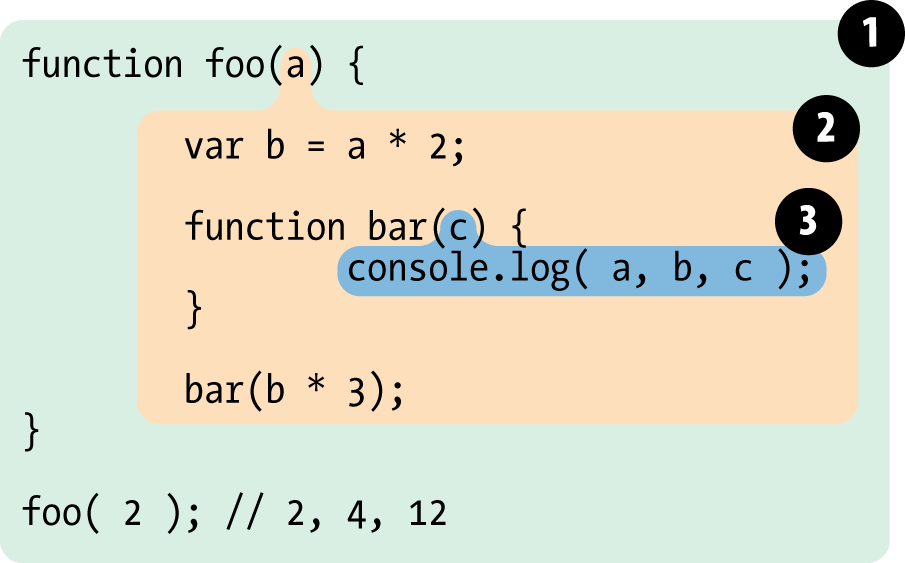
\includegraphics{fig2.png}
\caption{Nested scope \cite{getify}}
\end{figure}

The function \texttt{foo} is defined \emph{in} the global scope (1) (see
next section), and is therefore accessible from all parts of this
program. \texttt{foo} itself defines a new scope (2) which includes the
identifiers \texttt{a}, \texttt{b} and \texttt{bar}. \texttt{bar}
defines a new scope (3) within \texttt{foo}, defining only the
identifier \texttt{c}. As can be seen, the innermost scope (3) has
access to its own identifiers, as well as to the ones defined in its
containing scope (2).

\begin{quote}
Just as a block or function is nested inside another block or function,
scopes are nested inside other scopes. So,
\end{quote}

\subsubsection{Levels of scope}\label{levels-of-scope}

As mentioned above, the rules for when a new scope is defined differ
depending on the programming language. Usually, a language implements
multiple rules.

\begin{itemize}
\itemsep1pt\parskip0pt\parsep0pt
\item
  Functions define a new scope; blocks do not (in JavaScript)
\end{itemize}

\begin{description}
\item[Global scope]
Variables that are accessible from \emph{any point} in the program make
up the global scope.
\item[Block scope]
Any logical block, often denoted by containing curly braces (\texttt{\{}
and \texttt{\}}), will create a new scope. This is the case in the C
programming language, amongst others,
\item[Function scope]
Any function definition defines a new scope. Parameters of the function
are part of this newly defined scope.
\end{description}

In JavaScript, the run-time environment defines what is in the global
scope. The JavaScript engines in web browsers usually provide access to
the \ac{dom} through the \texttt{document} object, whereas Node.js
provides the \texttt{require} function to include CommonJS-style
modules.

In contrast, the Java programming language implements block scope, but
no global scope.

\subsubsection{Common scoping problems}\label{common-scoping-problems}

The following are common phenomena that arise through scoping and may be
the cause of problems. Though being typical for JavaScript, many of
those problems can arise in other programming languages, in the same or
similar form, as well.

These phenomena can generally be helpful or hindering, and thus be
desired or undesired. The goal of the concept developed in this thesis
is to make the developer recognize those phenomena during author-time,
and thus avoid confusion and reduce errors.

\begin{description}
\item[Hoisting]
is the implicit process, as done by the JavaScript engine, of moving
variable and function declarations „from where they appear in the flow
of the code to the top of the code“ \cite{getify}. By code,
\citename{getify} refers to the scope block. Any variable declaration
inside a scope block is hoisted to the top of the scope block.

\begin{verbatim}
        function foo() {
          a = 2;
          var a;
          console.log( a );
        }
\end{verbatim}

The above code is actually processed as:

\begin{verbatim}
        function foo() {
          var a;
          a = 2;
          console.log( a );
        }
\end{verbatim}

The variable declaration of \texttt{a} is moved, or „hoisted“, to the
top of the scope block of \texttt{foo}. Hoisting can impose unexpected
behaviour, especially when declaring variables of the same name in
nested scopes.
\item[Closures]
are a common phenomenon in JavaScript programs, but are more widely used
than they are understood. Citing \citename{getify}, closure is „when a
function is able to remember and access its lexical scope even when that
function is executing outside its lexical scope.“ \citeyear{getify} As
functions are first-class objects in JavaScript, they can be passed
around like variables, for example as callbacks. A function can also
return another function. But, as JavaScript works with \emph{lexical
scope} and, according to the nesting rules presented before, a function
must always have access to its ancestor scopes, an instance of the whole
scope chain is returned or passed along with the function. In other
words, the function „closes“ or „forms a closure“ over its ancestor
scopes. This may impact performance, as the closed-over scopes have to
stay in memory as long as a reference to the closure exists. It may also
lead to unexpected behaviour, for example if a variable defined outside
of a closure is used inside of it (see \citeasnoun*[Ch. 5]{getify} for
more examples).
\item[Shadowing]
is a consequence of nested scopes. If a variable (1) is defined in a
containing scope, and a new variable (2) of the same name is defined in
a contained scope, the contained scope has no access to (1). Variable
(1) is \emph{shadowed} by variable (2). As with all of the phenomenons
listed here, this can either be desired or unwanted behaviour. In the
code example below, shadowing the variable \texttt{i} would have
prevented an infinite loop. A good solution to avoid shadowing is
choosing different variable names throughout nested scopes.
\item[Implicit variable declaration]
JavaScript allows for the creation of variables and object properties in
an implicit way (\emph{silently}).
\item[Lookup performance]
The variable lookup through scope chains, as described above, can have
impact on the performance of an application.
\end{description}

Gutes Problem, dass durch mein Konzept gelöst werden könnte (führt zu
infiinite loop)

\begin{verbatim}
function foo() {
    function bar(a) {
        i = 3; // changing the `i` in the enclosing scope's for-loop
        console.log( a + i );
    }

    for (var i=0; i<10; i++) {
        bar( i * 2 ); // oops, inifinite loop ahead!
    }
}

foo();
\end{verbatim}
